\documentclass{article}
\usepackage{geometry}[left=1cm,right=1cm]
\usepackage{eso-pic,graphicx} % Required for inserting images

\title{ Nalfeshnee\\
    \large The Scourge of Tricorner}
\date{}


\begin{document}
    \AddToShipoutPictureBG{\includegraphics[width=\paperwidth,height=\paperheight]{../../Y7.png}}

    \maketitle
    
    \begin{figure}[h]
        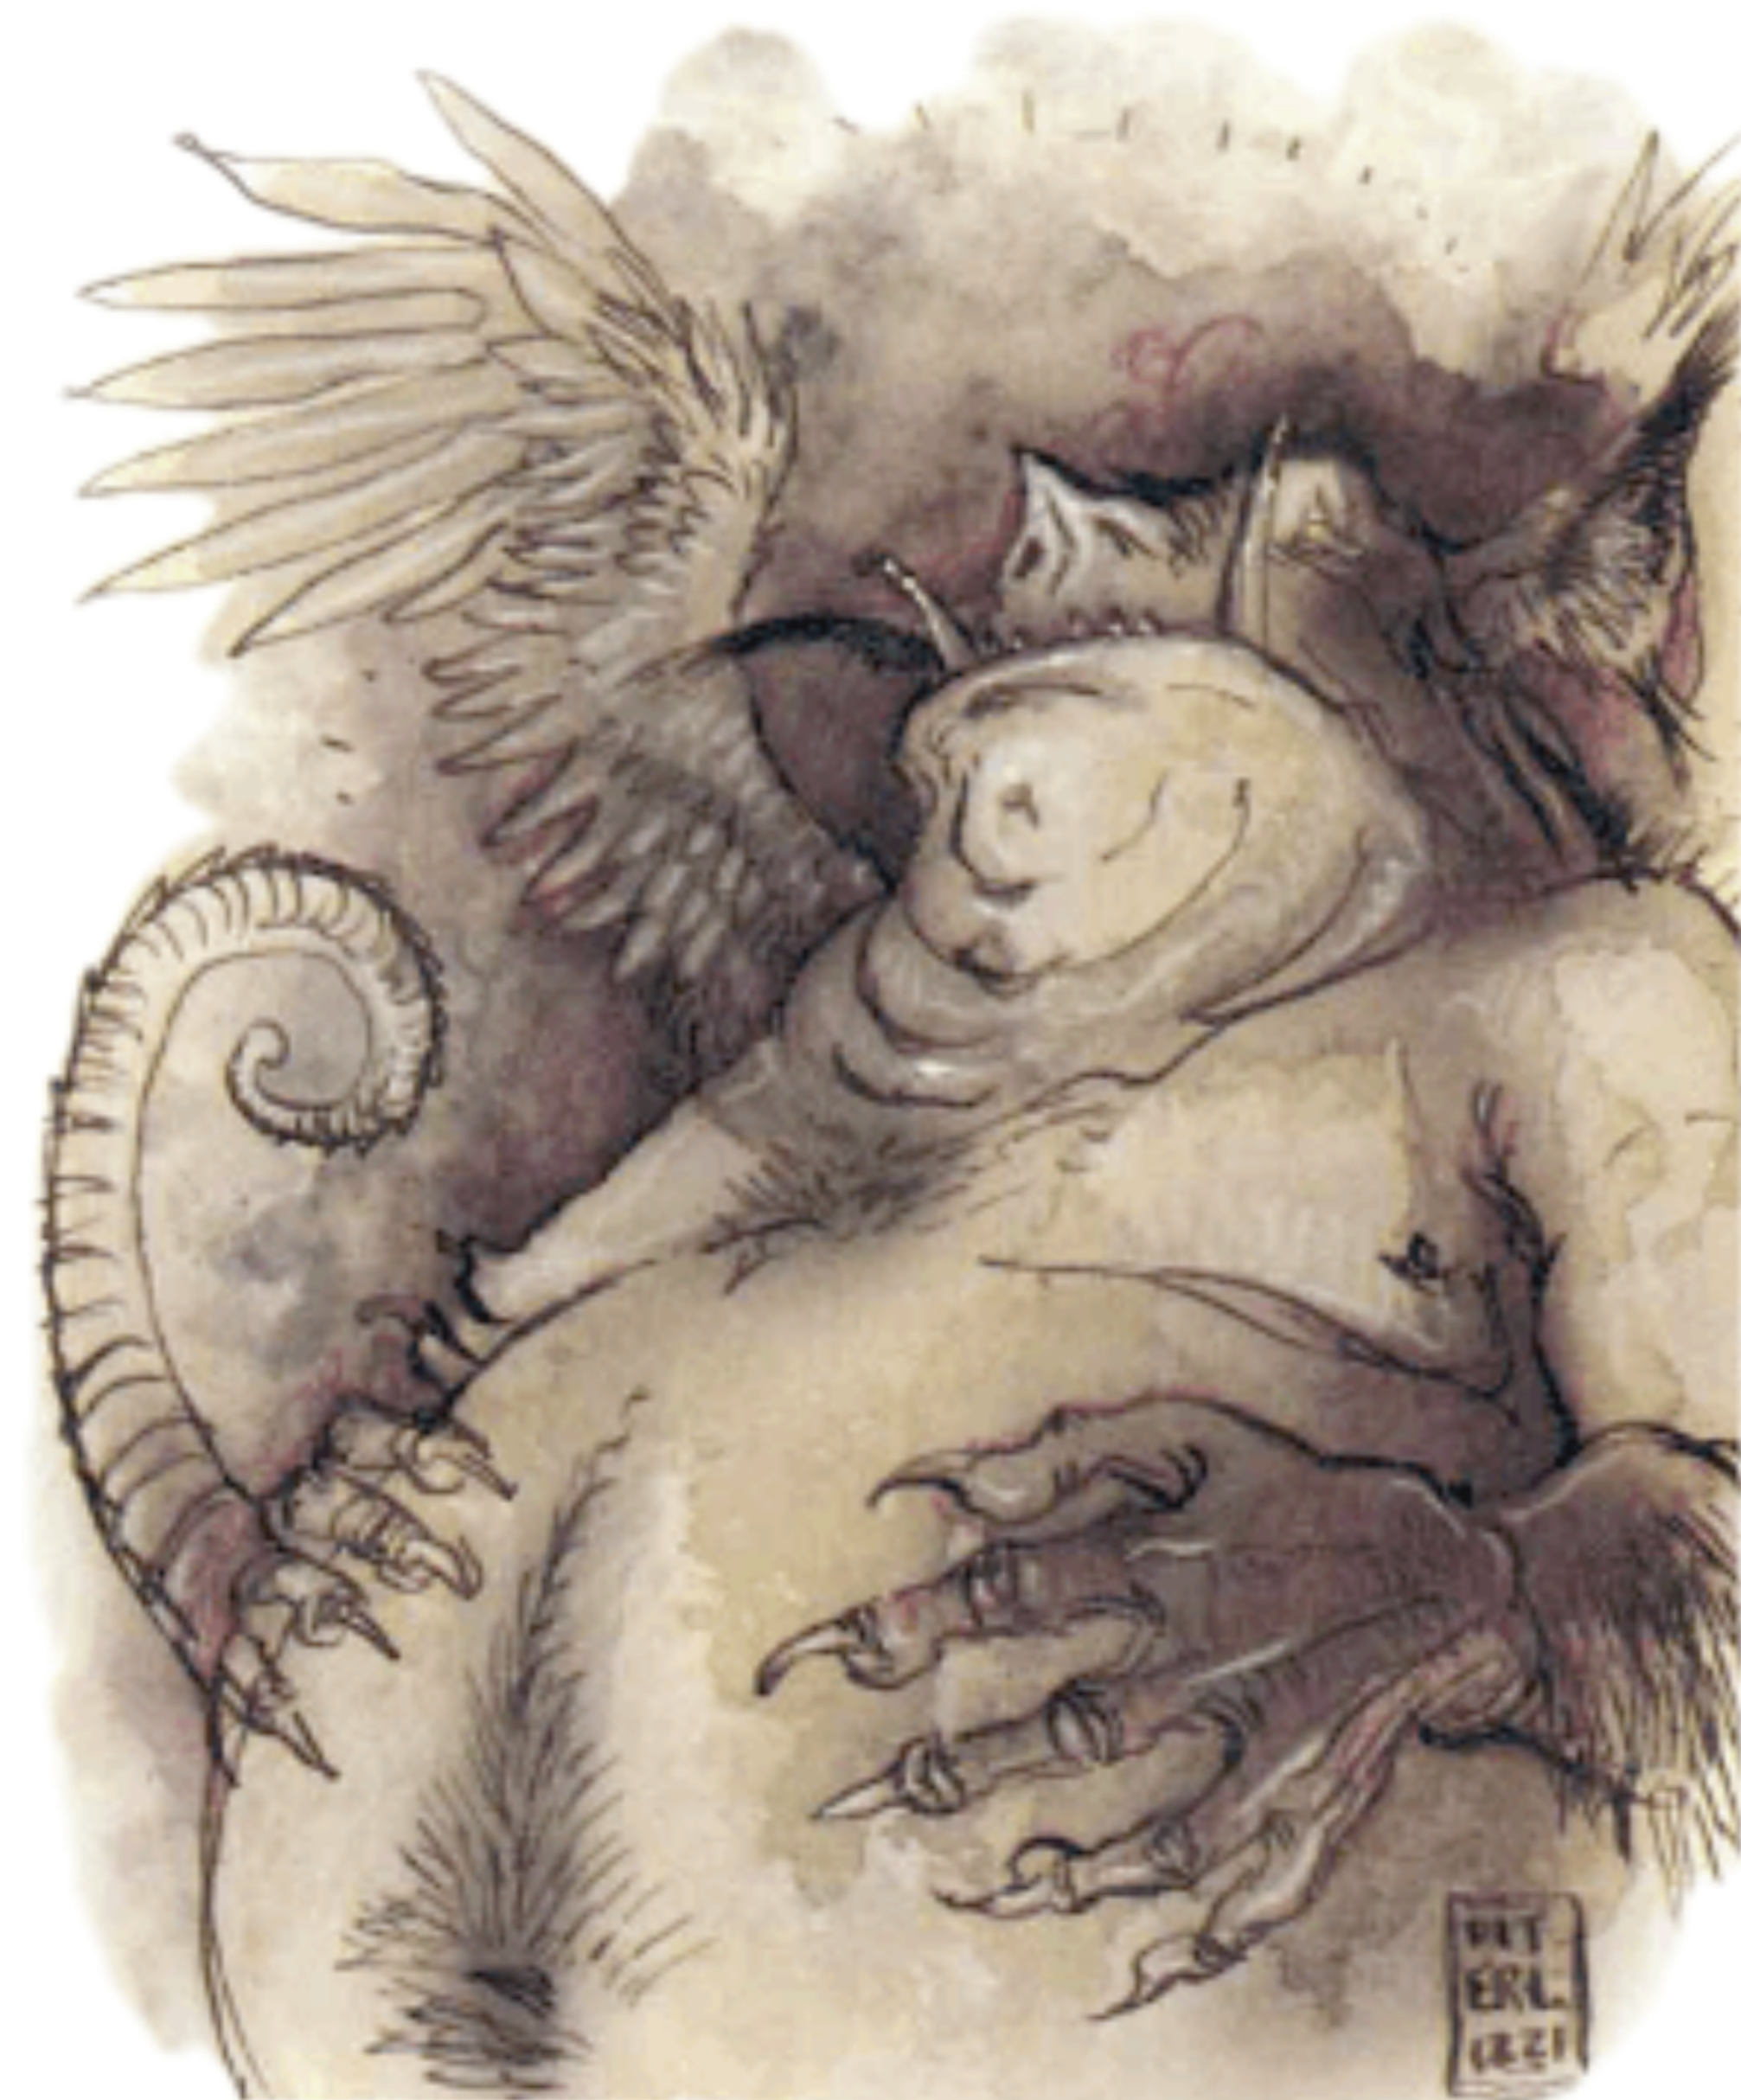
\includegraphics[width=8cm]{./tanatnal.png}
        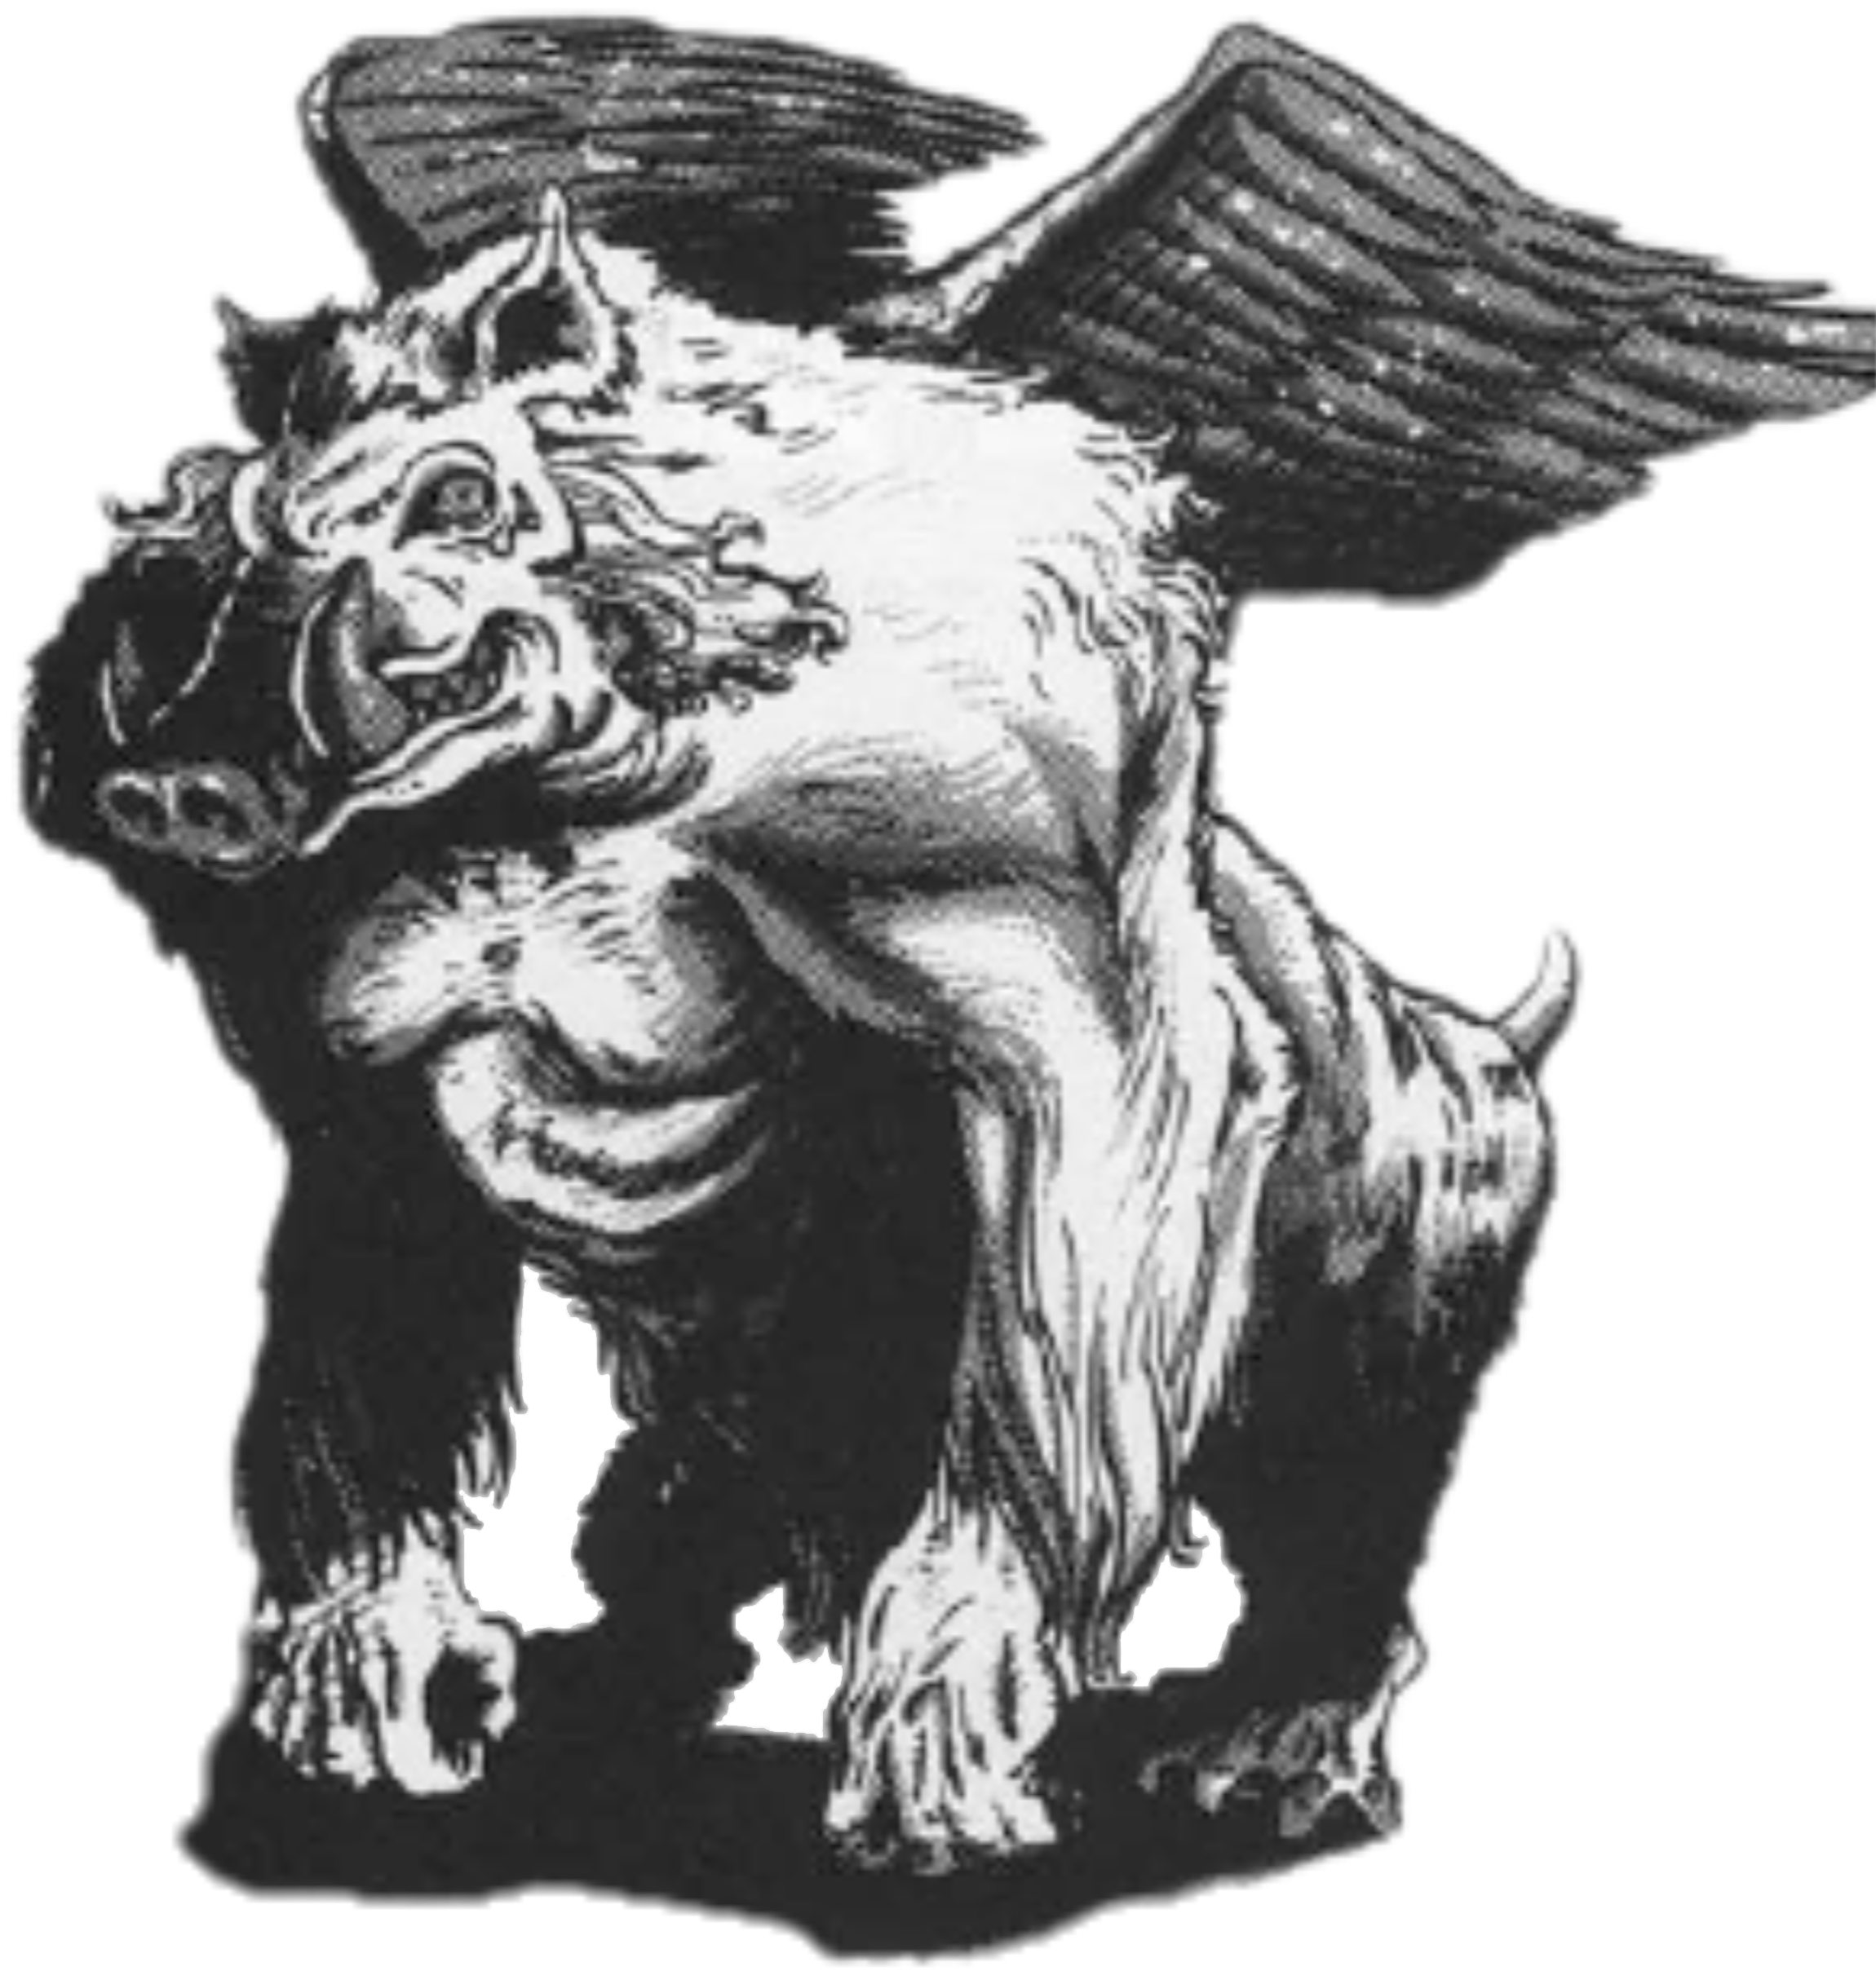
\includegraphics[width=8cm]{./nalfeshnee.png}
    \end{figure}

    \section*{Physical characteristics}

    Nalfeshnee are 20' tall; most of their immense strength goes simply to support their bodies. 
    They combine the worst features of ape and boar, and their small wings appear unable to bear their ponderous bodies. 
    Nalfeshnee have red, glowing eyes that pierce the mind and seem to draw energy from just a glance.

    \section*{Strengths}
    Its hide is as strong as plate mail and capable of with its tusks or claws to rend any of us in two within less than 10 seconds if given the chance.

    Its anatomy keeps it from being affected by most conventional poisons and toxins. It also shrugs off most elemental damage, focus on Percussive, planar, mental, acidic or force attacks. 
    Due to its extra planar existence, it is less affected by the magicks over all. Expect trying influence it directly with magic to fail. 

    It is claimed to be able to suffuse the surrounding air with lights which invades your minds and triggers a fear response. 
    The humanoid mind is able to recognize the pattern after being affected by it once so repeat attacks are unlikely 
    \section*{Weaknesses}
    Its greatest weakness is to my summation is its speed and agility. Its tiny wings can carry it at a regular pace but on the ground it's slower than that. 
    It is able to use magic to teleport which makes up for its slow canter, though it takes time to do so and should be obvious. Magic circles should make it difficult to do such.

    \section*{Strategy}

    A magic circle will be erected around Mr Silas Farsett. He will be summarily executed, releasing the Demon from within. 
    His body will be moved out of the magic circle and I, Paige Willowbranch will capture his soul after the demon has been released. Thus allowing for the safe resuscitation of him post combat. 

    All participants ought to stand more than 40ft away from the demon at all times, forcing it to close the distance by movement or teleportation, either lessens its threat potential.

    Ranged weapons are to be preferred due to the former point, these weapons must be enchanted or its ammunition to be at the very least. Spell casters are to focus on burst type spells of Acid, Physical, Force, Necrotic, Psychic, Radiant, Thunder varieties, summoning magics or targeting its agility over other defences if needed. 









\end{document}